\section{Introduction}
\label{sec:intro}

\begin{figure*}[t]
    \centering
    % \vspace{-2ex}
    \begin{subfigure}[t]{0.49\linewidth}
        \centering
        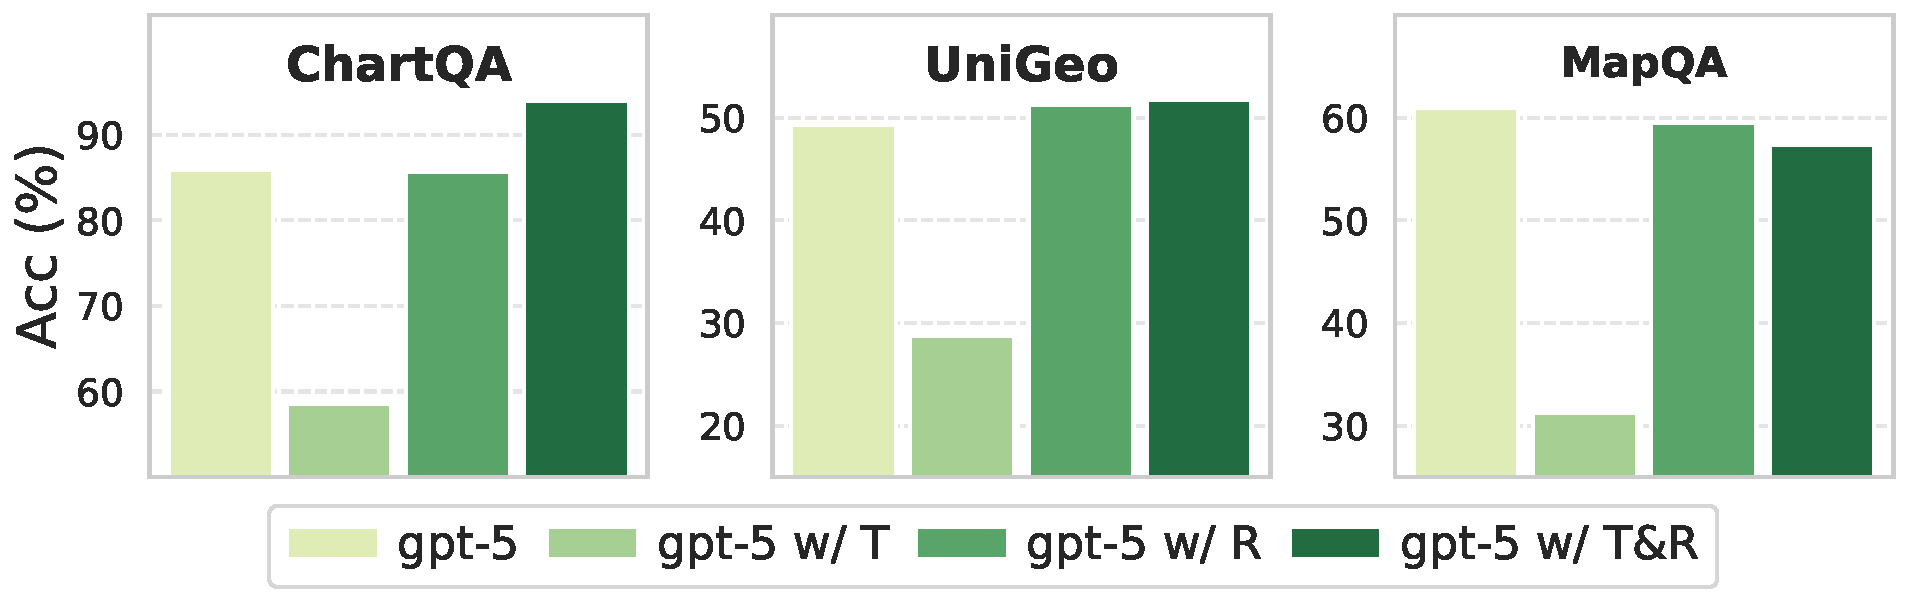
\includegraphics[width=\linewidth]{figure/fig1-1.pdf}
        \caption{Close-source VLM (\texttt{gpt-5}).}
        \label{fig:teaser-gpt}
    \end{subfigure}
    \hfill
    \begin{subfigure}[t]{0.49\linewidth}
        \centering
        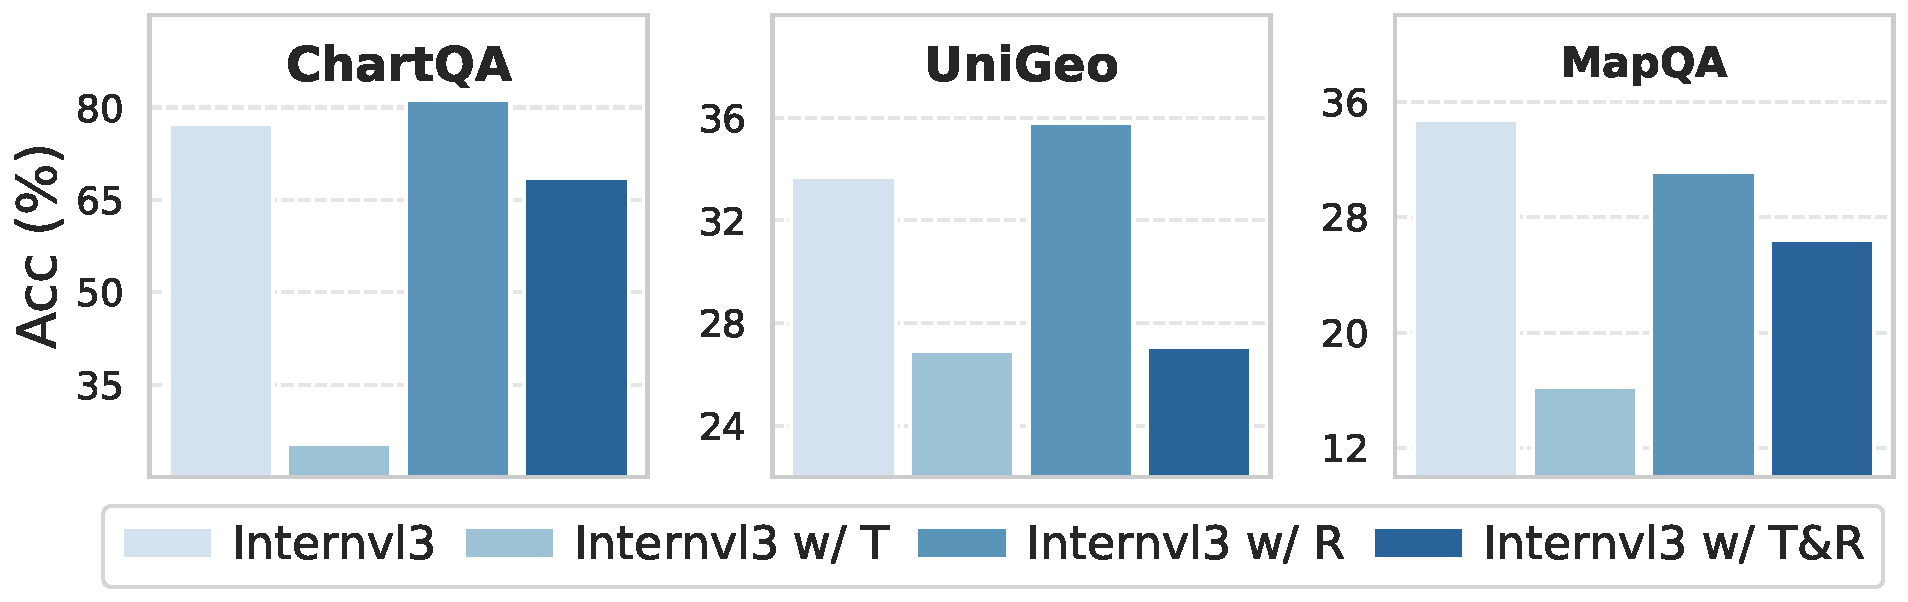
\includegraphics[width=\linewidth]{figure/fig1-2.pdf}
        \caption{Open-source VLM (\texttt{Internvl3-8B}).}
        \label{fig:teaser-internvl}
    \end{subfigure}
    % \vspace{-1ex}
    \caption{Directly augmenting VLMs with tools significantly degrades accuracy (\emph{w/ T}), yet intrinsic reasoning offers limited gains on complex VQA (\emph{w/ R}). Supplying \emph{tool‑selection prior knowledge} and interleaving reasoning with tool execution improve performance (\emph{w/ T\&R}); gains are task‑dependent for commercial VLMs, while small open‑source VLMs remain particularly struggling. }
    % \vspace{-2ex}
    \label{fig:teaser}
\end{figure*}


Recent progress in VLMs has demonstrated strong performance across tasks such as visual question answering, multimodal reasoning, and grounded mathematical problem solving~\citep{bai2025qwen2,guo2025integrating,dong2025insight,thawakar2025llamav}. 
Many of these advancements stem from incorporating text-based reasoning paradigms, particularly the Chain-of-Thought (CoT)~\citep{wei2022chain} and reinforcement learning (RL)~\citep{guo2025deepseek}, which decomposes complex tasks into intermediate text reasoning steps for problem solving, and leverages outcome-based rewards to refine reasoning quality~\citep{liu2025visualrft,huang2025vision,qi2024cogcom,liu2024chain,zhang2025chain,shen2025zoomeye,liang2025modomodo,shen2025vgent}.

Most of the existing VLM reasoning processes still rely on static visual embeddings and shallow cross-modal alignment. As a result, their text-only reasoning struggles to capture the fine-grained visual structures, spatial relationships, and quantitative dependencies present in real-world scenes~\cite{zheng2025deepeyes, fan2025grit}.
These limitations underscore the need for thinking-with-image paradigms~\cite{su2025thinking}, where reasoning is tightly coupled with visual perception, enabling richer cross-modal interaction and step-by-step visual reasoning.

To enhance visual-centric reasoning and encourage \emph{thinking-with-image} behaviors in VLMs, tool-integrated reasoning (TIR)~\citep{guo2025beyond,zheng2025deepeyes,xu2025incentivizing} has been introduced recently. TIR equips models with external tools, such as \emph{grounding}, \emph{zoom-in}, and \emph{search}, to facilitate fine-grained perception and reasoning over object interactions.
Despite its promise, current open-sourced VLMs still remain inadequate at leveraging these tools for effective reasoning, as shown in Figure~\ref{fig:teaser}.
This limitation highlights the urgent need for an effective training environment and strategies to \emph{select, invoke, and coordinate} visual tools dynamically. 
While there are several studies dedicated to improving tool usage capabilities for VLMs~\citep{wu2025mmsearchr1,zheng2025deepeyes,fan2025grit,su2025openthinkimg}, those works are often narrow in scope, often confined to specific tasks (\eg, using image search for knowledge or zoom-in for object grounding). 
In parallel, recent efforts in gaming and robotics~\citep{chen2025g1,wang2025vagen} have introduced unified environments for training VLM agents. These platforms provide controllable dynamics, grounded feedback, and structured task spaces, offering clear advantages for robot learning and conceptually aligning with TIR. 
However, the simulation of tool-integrated thinking in VLMs—especially for open-domain visual reasoning—remains largely underexplored.

Motivated by these challenges, we introduce \env{} (\textbf{Vis}ual-centric \textbf{T}ool-integrated \textbf{A}gentic training environment), a scalable, agentic training environment designed to systematically enhance the reasoning and decision-making capabilities of VLM agents across complex, real-world scenarios. Specifically, \env{} wraps up visual tool operations and provides textual feedback on receiving tool call commands by VLMs, and features:
\begin{itemize}[leftmargin=*,noitemsep,topsep=2pt]
    \item \textbf{Diverse multi-modal reasoning tasks.} \env{} provides a comprehensive VQA suite spanning 7 reasoning tasks across 13 public datasets, supporting training and evaluation of agents with strong generalization and tool‑integration skills.  
    \item \textbf{Unified, extensible tool interface.} \env{} exposes a standardized API over 26 pre‑defined tools that support perception, symbolic manipulation, chart and document interpretation, grounding high‑level reasoning in structured intermediate results. 
    \item \textbf{Scalable interactive infrastructure.} \env{} accelerates agent training via multithreading, parallel execution, and sequential sampling, enabling efficient trajectory collection and large‑scale automated evaluation compatible with diverse agent scaffolds.  
\end{itemize}
Building on \env{}, we further develop \ours{}, a VLM-based agent trained for robust, tool-augmented reasoning. Across five in‑domain and six out‑of‑domain reasoning‑intensive VQA benchmarks, \ours{}‑8B surpasses state‑of‑the‑art open‑source baselines of comparable size by 9.51\%–18.72\%. \env{} proves to be an effective and scalable solution for developing VLM agents that can robustly interleave reasoning and tool use to solve complex, multi-step visual problems.
